\chapter{Static Analysis Tools}

% TODO: https://en.wikipedia.org/wiki/Static_program_analysis Cite an article from here maybe
Static program analysis is the process of automatically analysing source code to extract information about its behavior without executing it \todo{cite}, as opposed to dynamic analysis, which is performed on programs as they are run.
Static analysis tools can ease the burden of software development by automating tasks that would otherwise require manual effort and meticulous attention to detail.
These tools can perform a variety of tasks, ranging from detecting possible bugs \cite{johnson_lint_1978,hovemeyer_finding-bugs_2004} to formal sound verification of program properties \cite{blanchet_static-analyzer_2003}.

Static analysis tools are increasingly becoming more important in modern software development, as modern code continues to become more complex and difficult to reason about.
Industry leaders, such as Google \cite{sadowski_analysis-google_2018} and Meta (formerly Facebook) \cite{calcagno_moving-facebook_2015}, have embraced static analysis tools as integral components of their software development workflows.

% TODO: IDE integration

\section{Purposes of Static Analysis Tools}
Typically in a software development workflow, multiple static analysis tools are used in conjunction to provide a comprehensive suite of checks. % TODO: often these are bundled in the IDE as plugins etc.
These tools enable the developer to perform a variety of tasks and activities to aid them in writing idiomatic code.

A point of confusion is that many modern static analysis tools may perform multiple of these activities, and as such, terms referring to such activities are often used interchangeably.
This section aims to establish definitions for some of these tasks, which will be used as a basis for subsequent discussion within this thesis.
However, it is important to remember that the boundaries between them can be blurry.

\subsection{Linting}
\textbf{Linting} is the process of analysing source code to identify and report issues related to coding style, formatting, and potential programming errors.
The term originates from the \texttt{lint} program \cite{johnson_lint_1978}, which examined C source code for bugs, as well as wasteful code patterns that are legal but error-prone.
The tool was also utilised to enforce portability restrictions which aided users in writing portable code that could be compiled on multiple platforms.
Since the release of \texttt{lint}, many linting tools, known as \textbf{linters}, have been developed for a wide range of programming languages.

Linters are provided as standalone tools rather than as part of a compiler, since their primary goal is to suggest improvements for code readability and maintainability, rather than code optimisations.
The majority of modern-day linters are integrated into code editors and \textsc{ide}s as plugins, allowing them to provide real-time feedback to developers as they write code.
Code analysis performed by the linter is run incrementally in the background and then displayed directly in the editor.
This enables developers to make informed decisions while writing code, rather than having to run the linter as part of compilation or as an extra step in their workflow.

% TODO: Clippy for Rust https://arxiv.org/abs/2310.11738
Within the editor, linters can highlight problematic snippets of code and in some cases can offer relevant recommendations to fix them.
This is achieved by detecting suspicious code patterns that may be indicative of possible bugs or poor coding practices: these are commonly referred to as \textbf{code smells} \cite{fowler_refactoring_2018}.
% TODO: https://checkstyle.sourceforge.io/
Furthermore, linters are also used as style checkers to enforce coding standards and best practices \todo{cite CheckStyle, ESLint?}, ensuring that code is idiomatic, readable, and consistent across a codebase.
Some linters may also provide automated code transformations to fix formatting issues or style violations that they detect.
An example of a linter providing a warning and automated code fix to help improve code style is shown in fig.~\ref{fig:hlint-example}.

\begin{figure}[htbp]
  \vspace{3ex} % TODO: make this less hacky
  \centering
  \begin{subfigure}{0.45\textwidth}
    \centering
    \begin{minted}[frame=single]{haskell}
      foo xs = map (+1) xs
    \end{minted}
    \caption{A Haskell function \texttt{foo}, which can be made more concise using $\eta$-reduction.}
  \end{subfigure}
  \hfill
  \begin{subfigure}{0.45\textwidth}
    \centering
    \begin{minted}[frame=single,escapeinside=||]{text}
      Eta reduce
      Found:
        foo xs = map (+ 1) xs
      Why not:
        foo = map (+ 1)
      |\textcolor{gray}{hlint(refact:Eta reduce)}|
    \end{minted}
    \caption{The linter warning shown for \texttt{foo}.}
  \end{subfigure}
  \caption{An example of a warning from the Haskell linter \texttt{hlint} \cite{mitchell_hlint_2024}, suggesting a fix that a user can choose to automatically apply.}
  \label{fig:hlint-example}
\end{figure}

\subsection{Automated Refactoring}
Code refactoring is a well-established practice in software development.
In his influential book \textit{Refactoring: Improving the Design of Existing Code} \cite{fowler_refactoring_2018}, Fowler defines \textbf{refactoring} as ``the process of changing a software system in such a way that it does not alter the external behavior of the code yet improves its internal structure''.
In essence, refactoring is a particular type of code restructuring that improves its design and eliminates code smells while preserving behaviour.

Static analysis tools can reason about how to safely refactor code in an automated manner, performing refactorings as source-to-source transformations.
This is particularly useful for large codebases, where manual refactoring would be tedious and error-prone.
Fig.~\ref{fig:extract-function-intellij} presents \textit{Extract Function}, an example of a common refactoring that can be performed automatically, where a block of code is extracted into its own function.

\begin{figure}[htbp]
  \centering
  \begin{subfigure}{\textwidth}
    \centering
    \begin{minted}[frame=single,highlightlines={4-5},linenos]{scala}
      object Main {
        def main(args: Array[String]): Unit = {
          val bankDetails = getBankDetails()
          println(s"Account name: ${bankDetails.name}")
          println(s"Account balance: ${bankDetails.balance}")
        }
      }
    \end{minted}
    \caption{A snippet of Scala code. A user may wish to extract the highlighted lines into a separate function.}
  \end{subfigure}
  \begin{subfigure}{\textwidth}
    \centering
    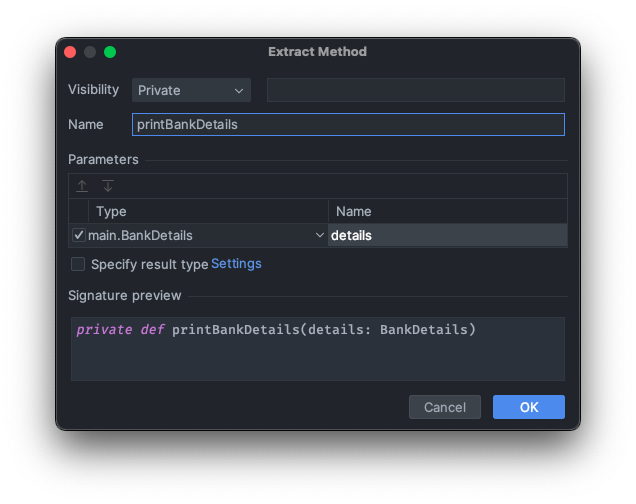
\includegraphics[width=0.75\textwidth]{background/extract-function-intellij.png}
    \caption{A refactoring dialogue for the \textit{Extract Function} refactoring in IntelliJ IDEA, which can be opened within the available refactorings by selecting the highlighted lines.}
    \label{fig:extract-function-intellij-dialogue}
  \end{subfigure}
  \begin{subfigure}{\textwidth}
    \vspace{3ex} % TODO: ew
    \centering
    \begin{minted}[frame=single,highlightlines={4,7-10},linenos]{scala}
      object Main {
        def main(args: Array[String]): Unit = {
          val bankDetails = getBankDetails()
          printBankDetails(bankDetails)
        }

        private def printBankDetails(details: BankDetails): Unit = {
          println(s"Account name: ${details.name}")
          println(s"Account balance: ${details.balance}")
        }
      }
    \end{minted}
    \caption{The result of applying the \textit{Extract Function} refactoring using the chosen parameters in fig.~\ref{fig:extract-function-intellij-dialogue}.}
  \end{subfigure}
  \caption{An example of the \textit{Extract Function} refactoring in IntelliJ IDEA \cite{jetbrains_intellij_2021}.}
  \label{fig:extract-function-intellij}
\end{figure}

Generally, when a user makes use of an automated refactoring tool in an \textsc{ide}, they will manually identify the snippet of code that they wish to refactor, and then select the appropriate refactoring from a list of available options.
Linters can also aid in the refactoring process by identifying candidate areas for refactoring and suggesting appropriate actions that the user can take.

Given that many linters can perform automated code transformations, the distinction between refactoring and linting can be confusing.
We make the key distinction that linting is concerned with the \textit{detection} of issues in code, while refactoring is concerned with \textit{transforming} code to avoid some of these issues.
When linters apply automated code transformations to fix issues, some of these transformations may be considered refactorings.
Thus, many static analysis tools provide both linting and refactoring functionalities.
For example, when a linter detects a fragment of code that is repeated in multiple places, it may suggest the \textit{Extract Function} refactoring to avoid code duplication.
The linting tool itself may provide the automated refactoring functionality to perform the transformation.
The $\eta$-reduction example in fig.~\ref{fig:hlint-example} is another example of a refactoring suggested by a linter to conform to an idiomatic Haskell style.
We see that \texttt{hlint} can both highlight the issue to the user and perform the suggested refactoring automatically.

\subsection{Bug Fixing / Automated Program Repair}
% As opposed to linters they use more advanced static analysis techniques?
% These terms are pretty conflated tbh

% Outline
% * Static analysis tools for general guidance as well as domain-specific guidance for libraries
% * Static analysis tools help developer productivity, as well as guiding best practices, whether for a programming language in general or a specific problem domain when working with a library
% * Examples of types of activities that static analysis tools may do, including linting, refactoring, bug fixing, and formal verification (the last is out of scope for the project)
% * How these static analysis tools may be integrated in an IDE with code actions
% * How such tools are implemented, traversing the AST, etc.

\chapter{Parser Combinators}
